%! TEX root = ../main.tex
\section{The {\gerda} dataset and Monte Carlo simulations}\label{sec:data}
% {{{ THE GERDA DATA STRUCTURE
\marginnote{the\\{\gerda}\\data\\structure} In general the binary raw data format is custom defined by the different data acquisition systems. In order to optimize the analysis streaming and to provide a unique input interface for the analysis, all raw data are converted to a common standardized format. MGDO \cite{MGDO} (\textsc{Majorana} {\gerda} Data Objects) is a software library jointly developed by {\gerda} and \textsc{Majorana} \cite{majoranadem}. The core function of this software is to provide a collection of \texttt{C++} objects to encapsulate HPGe detector array event data and related analytical quantities. It also includes implementations of a number of general-purpose signal processing algorithms to support advanced detector signal analysis. The custom data objects available in the MGDO package are used as reference format to store events, waveforms, and other DAQ data (time stamps, flags). The MGDO data objects are stored as ROOT \cite{ROOT} files. The set of ROOT files produced by the conversion of raw data is named \textsc{Tier1}, and is officially distributed for the analysis.

Since the information contained in the \textsc{Tier1} set and in the raw data is expected to be equal, the conversion procedure is the optimal place where blinding can be applied. Events with an energy within $\pm$25 keV around $Q_{\beta\beta}$ are not exported to \textsc{Tier1} but they remain saved in the backup of the raw data.

The software framework \textsc{Gelatio} \cite{GELATIO} contains nearly independent and customizable modules that are applied to the input \textsc{Tier1} waveforms. The results (pulse amplitude, rise time, average baseline, energy, etc.) are stored as a new ROOT file (\textsc{Tier2}). A description of the analysis modules is presented in Ref.~\cite{dataproc}. Higher level \textsc{Tier}\emph{i} files that contain additional parameters evaluated from more advanced analysis (e.g.~calibrated energy spectra) can be created. In principle only the \textsc{Tier1} is official and every analysis should produce his own \textsc{Tier2} files depending on the actual needs. However there exists a `reference' \textsc{Tier2} produced with a standard set of \textsc{Gelatio} modules with a reasonable choice of parameters (e.g.~the width of the gaussian filter responsible for the reconstruction of the energy of an event) that can be used in most situations. The same reference datasets are provided for every \textsc{Tier}\emph{i} level.

Once the relevant quantities have been extracted from raw waveforms they have to be calibrated (e.g.~energy) and quality cuts (e.g.~to reject unphysical events) have to be applied. The results are again stored as a ROOT file (\textsc{Tier3}). The extraction of parameters related to the entire event (e.g.~the number of channels with a physical signal) is also performed at this level. Finally, high-level quality cuts are applied in \textsc{Tier4}, such as pulse shape discrimination, muon-veto and LAr-veto.

% }}}
% {{{ QUALITY CUTS
\marginnote{quality\\cuts} The data selection procedure undergoes various steps in order to purify the dataset from unphysical or unwanted events. Tn the following the different classes of events excluded from the analysis is presented.
\begin{itemize}
	\item There is a set of classes of events that originates from failures in the acquisition process, limitations of the hardware components (e.g.~the FADC) or failures in the reconstruction process (\textsc{Gelatio}).
	\item There are events not related to an energy deposition, and thus consisting of a flat signal (an energy deposition in one detector triggers the sampling of the pulses from each of the 40 detectors, so it is very common to find pure-baseline signals in data), waveforms which amplitude exceeds the FADC's energy threshold (overshoot events), pile-up events, and all other unphysical events.
	\item The main purpose for acquiring pulses from all the detectors when an energy deposition occurs anywhere is to provide the ability to discriminate multi-detector events. Such events cannot be associated to the double-beta decay electrons, which are absorbed within the detector's volume, and thus they can be discarded as background events.
	\item Events that leave a trace also in the water tank and/or in the upper scintillating panels and thus flagged by the muon-veto system are also discarded.
\end{itemize}

% }}}
% {{{ THE ENERGY SPECTRA
\marginnote{the\\energy\\spectra} With the cuts described above, the summed energy spectra from BEGe, enriched coaxial and natural coaxial detectors are presented in Fig.~\ref{fig:data}. The considered data set was taken between December 2015 and March 2017. Some prominent features can be identified. The low energy part up to 565 keV is dominated by $\beta^-$ decay of cosmogenic \ce{^{39}Ar} in all spectra. Slight differences in the spectral shape between the coaxial and BEGe type detectors result from differences in detector geometry and of the n$^+$ dead layer thickness. Between 600 and 1500 keV the spectra of the enriched detectors exhibit an enhanced continuous spectrum due to $2\nbb$ decay (see also Fig.~\ref{fig:energyspectra}). In all spectra, $\gamma$ lines from the decays of \ce{^{40}K} and \ce{^{42}K} can be identified, the spectra of the enriched coaxial detectors contain also lines from \ce{^{208}Tl} and \ce{^{214}Bi}. The peak-like structure around 3.5 MeV can be attributed to the $\alpha$-decays near the detector p$^+$ surface.

% }}}
% {{{ BACKGROUND INDEX
\marginnote{background\\index} The Background Index (BI), used to estimate the background activity in the \textsc{RoI}, is defined as the number of counts over detector's mass, live time and energy range inside a energy window defined as follows (see also Fig.~\ref{fig:bi}). The window covers the energy range between 1930 keV and 2190 keV excluding the blinded window around $Q_{\beta\beta}$. Also the two lines from \ce{^{208}Tl} and \ce{^{214}Bi} occurring respectively at 2104 keV and 2119 keV are neglected in this computation. This is done removing the energy range within $\pm$5 keV around the peaks. The width of the window is then 190 keV. In Tab.~\ref{tab:bindex} the background indices for the three considered datasets are given.
\begin{table}[b]
	\centering
	\label{tab:bindex}
	\caption{Background indices for the considered datasets.}
	\begin{tabular}{lc}
		\toprule
		\multirow{2}{*}{\textsc{dataset}}	&	BI \\
											&	cts/(keV$\cdot$kg$\cdot$yr) \\
		\midrule
		BEGe								&	$2.9\cdot10^{-3}$	\\
		\textsc{enr coax}					&	$4.3\cdot10^{-3}$	\\
		\textsc{nat coax}					&	$6.9\cdot10^{-3}$	\\
		\bottomrule
	\end{tabular}
\end{table}

\begin{figure}
	\centering
	\includegraphics{img/bi.pdf}
	\caption{Energy window used to compute the background index, a 50 keV wide energy window around $Q_{\beta\beta}$ and two 10 keV wide energy windows around the \ce{^{208}Tl} and \ce{^{214}Bi} peaks are excluded. The displayed data correspond to the energy depositions from all the {\gerda} detectors.}
	\label{fig:bi}
\end{figure}
% }}}
\subsection*{Monte Carlo simulations}
\addcontentsline{toc}{subsection}{Monte Carlo simulations}
Background components that were identified in the energy spectra or that were known to be present in the vicinity of the detectors were simulated using the \textsc{MaGe} \cite{MaGe} code based on \textsc{Geant4} \cite{geant4} and jointly developed by the {\gerda} and \textsc{Majorana} \cite{majoranadem} collaborations. The detectors and the arrangement of the germanium detector array with seven detector strings were implemented into the \textsc{MaGe} code as well as the other {\gerda} components (see Fig.~\ref{fig:volumes}). During the simulation \textsc{Geant4} generates complete information about the trajectory and interactions of particles as they propagate through the detectors. Although all of this information is available to the user, it is typically processed, parsed and saved to an output file for further analysis after the simulation run is complete. Simulations of contaminations of the following hardware components were performed:
\begin{itemize}
	\item on the p$^+$ and n$^+$ surfaces of the detectors;
	\item homogeneously distributed in the LAr, in a {\color{red}???} cylinder centered in the detector array;
	\item in the detector assembly representing contaminations in the detector holders and their components;
	\item in the nylon mini-shroud surrounding the detectors;
	\item in the fiber shroud;
	\item in the high-voltage cables and the signal cables.
\end{itemize}
The volumes representing the germanium array, the holder mounting and the cables are simulated as depicted in Fig.~\ref{fig:volumes}. The mini-shroud volume is implemented as a set of cylinders surrounding each detector string, while the fiber shroud consists of the lateral surface of a cylinder.
\begin{figure}
	\centering
	\resizebox{\textwidth}{!}{%
		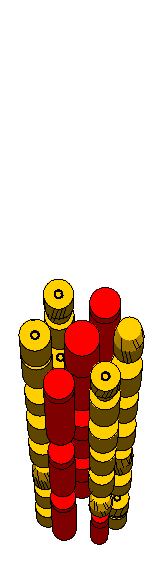
\includegraphics[]{img/gedet.pdf}%
		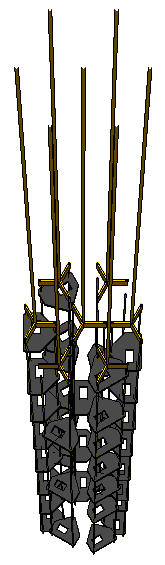
\includegraphics{img/holders.pdf}%
		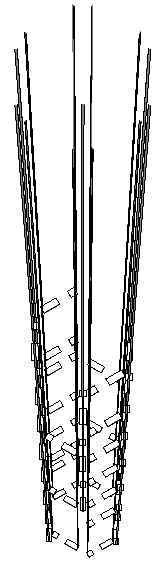
\includegraphics{img/cables.pdf}%
		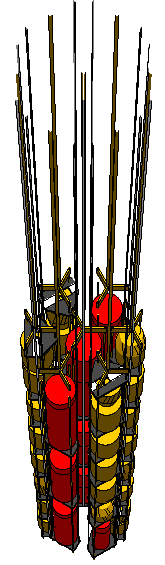
\includegraphics{img/all.pdf}%
	}%
	\caption{Implementation of the simulated volumes in \textsc{MaGe}. From left to right: the germanium detectors, the holder mounting, the cables and the three volumes put together.}\label{fig:volumes}
\end{figure}

% {{{ muons, neutrons, water tank
The expected background indices due to the neutron and muon fluxes at the LNGS underground laboratory have been estimated to be of the order < $10^{-5}$ cts/(keV$\cdot$kg$\cdot$yr) \cite{neutronsBI} and < $10^{-4}$ cts/(keV$\cdot$kg$\cdot$yr) \cite{muonsBI} respectively, and then are not considered. It has been also shown in earlier works that the contributions of the cryostat and water tank components are of the order < $10^{-4}$ cts/(keV$\cdot$kg$\cdot$yr) \cite{criowaterBI}, and then they have not been considered in this analysis.

% }}}
% {{{ 2nbb
\marginnote{$2\nbb$} The spectrum of the two electrons emitted in the $2\nbb$ decay of \ce{^{76}Ge} is sampled according to the distribution of \cite{tables2nbb} that is implemented in the code \textsc{Decay0} \cite{decay0}. The $2\nbb$ decay distributions of \cite{tables2nbb} are in principle more precise than those based on the Primakoff-Rosen approximation, and they have been cross-checked against the high-statistics data of the \textsc{Nemo} experiment for several nuclei \cite{nemo1,nemo2,nemo3,nemo4,nemo5}. Electrons are propagated in the {\gerda} simulated setup by \textsc{MaGe} and the total energy released in the active mass of the enriched detectors is registered.

% }}}
% {{{ 42Ar
\marginnote{\textnormal{\ce{^{42}Ar}}} While the distribution of \ce{^{42}Ar} is homogeneous inside LAr, the short lived ionized decay product \ce{^{42}K} ($T_{1/2} = 12.3$ h) can have a significantly different distribution due to drifts of the \ce{^{42}K} ions inside the electric fields that are present near the detectors. Separate spectra for two \ce{^{42}K} distributions have thus been simulated: homogeneous in LAr in a volume of centered around the full detector array, on the n$^+$ and on the p$^+$ detector surface of the detectors. As the spectral shape is not expected to vary strongly between the detectors, the isotope on the n$^+$ and p$^+$ surface was simulated only for a single detector. The simulated spectral shapes are shown in Fig.~\ref{fig:simspectra}.

% }}}
% {{{ 238U
\marginnote{\textnormal{\ce{^{238}U}}-chain} \ce{^{214}Bi} and \ce{^{214}Pb} are the only one in the \ce{^{226}Ra} $\rightarrow$ \ce{^{210}Pb} sub-chain decaying by $\beta$ decay accompanied by emission of high energy $\gamma$ particles and they are assumed to be in equilibrium. \ce{^{214}Bi} and \ce{^{214}Pb} were simulated in the holder mounting, in the cables, in the fiber shroud and in the mini-shrouds. For the \ce{^{238}U} $\rightarrow$ \ce{^{226}Ra} the \ce{^{234\text{m}}Pa} was simulated, as the $Q_\beta$ of \ce{^{234}Th} is below the considered fitting range. {\color{red}giustificazione da ampliare}

% }}}
% {{{ 232Th
\marginnote{\textnormal{\ce{^{232}Th}}-chain} The characteristic $\gamma$ line at 2615 keV, a hint of the presence of isotopes from the \ce{^{232}Th} chain, can be clearly identified in the energy spectra shown in Fig.~\ref{fig:data}. Possible locations for contaminations are the detector assembly, the cables, the mini-shrouds and the fiber shroud. As \ce{^{228}Ac} and \ce{^{228}Th} do not necessarily have to be in equilibrium, the two parts of the decay chain were simulated separately. From the sub-decay chain following the \ce{^{228}Th} decay only the contributions from the \ce{^{212}Bi} and \ce{^{208}Tl} decays were simulated, as theses are the only ones emitting high energetic $\gamma$ rays and electrons that can reach the detectors. {\color{red}giustificazione da ampliare}

% }}}
% {{{ 60Co
{\color{red}Manca 60Co}%\marginnote{\textnormal{\ce{^{60}Co}}}

% }}}
% {{{ 207Bi
{\color{red}Manca 207Bi}%\marginnote{\textnormal{\ce{^{207}Bi}}}

% }}}
% {{{ ALPHA MODEL
\marginnote{$\alpha$-model} From energies above 3.5 MeV the spectrum is dominated by $\alpha$-decay events, thus the background model in this region has been developed independently and then the resulting energy distribution has been added as a single contribution among the other background contributions.

A strong contribution from \ce{^{210}Po} can be observed in Fig.~\ref{fig:data}. This is indication for a surface contamination of the detectors. However, there are also hints for other peak like structures at 4.7, 5.4 and 5.9 MeV that can be attributed to the decays of \ce{^{226}Ra}, \ce{^{222}Rn} and \ce{^{218}Po} on p$^+$ detectors surfaces, respectively.

Due to the short range of $\alpha$-particles in germanium and LAr of the order of tens of $\mu$m, only decays occurring on or in the close vicinity (few $\mu$m) of the p$^+$ surface (assumed dead layer thickness roughly 300 nm) can contribute to the measured energy spectrum as the n$^+$ dead layer thickness is roughly 1 mm. The energy deposited in the active volume of the detector by surface or close to surface $\alpha$-particles is very sensitive to the thickness of the dead layer and on the distance of the decaying nucleus from the detector surface.

All $\alpha$-decays in the \ce{^{226}Ra} to \ce{^{210}Pb} sub-decay chain and the \ce{^{210}Po} decay have been simulated on the p$^+$ detector surface separately. Additionally, the decays in the chain following the \ce{^{226}Ra} decay were simulated assuming a homogeneous distribution in a volume extending up to 1 mm from the p$^+$ surface in LAr. The individual decays on the p$^+$ surface result in a peak-like structure with its maximum at slightly lower energies than the corresponding $\alpha$-decay energy with a quasi-exponential tail towards lower energy. The decays occurring in LAr close to the p$^+$ surface result in a quasi-flat spectrum without any peak-like structure extending to lower energies.

The \ce{^{210}Po} peak structure around 5.3 MeV with high statistics was used to determine the effective dead layer model. Spectra from \ce{^{210}Po} $\alpha$-decay simulations on the p$^+$ surface with different dead layer thicknesses were used to fit the spectrum in the energy region dominated by the \ce{^{210}Po} peak, i.e.~between 4850 and 5250 keV. The weight of each spectrum was left as a free parameter. A combination of the spectra for 300, 400, 500 and 600 nm dead layer thicknesses describes the observed peak structure well and results in a good fit, whereas a spectrum with a single dead layer thickness does not give a sufficiently good fit. Consequently the derived dead layer model was used for the later fits of $\alpha$-induced spectra.

In order to describe the whole energy interval dominated by $\alpha$-induced events, the simulated spectra of $\alpha$-decays of \ce{^{210}Po} as well as from \ce{^{226}Ra} and its short lived daughter nuclei on the p$^+$ surface and in LAr were used to fit the energy spectrum between 3500 and 7500 keV. In fact, while the surface decays alone can successfully describe the observed peak structures, they could not describe the whole spectrum. A contribution from an approximately flat component, like the spectra from $\alpha$-decays in LAr, is needed in the model. The number of events in the considered energy range was left as a free parameter for each $\alpha$-component.

% }}}
\subsection*{Screening measurements}
\addcontentsline{toc}{subsection}{Screening measurements}
There are some radioactive contaminations in the components of {\gerda}, though not evident in the energy spectra, which have been identified and systematically measured. The most relevant contributions, reported in Table \ref{tab:screening}, come from the silicon of the holder mounting, the cables, the nylon mini-shroud covering the detectors and the fiber shroud.
\begin{table}
	\caption{Screening measurements for some of the considered {\gerda} components. The upper limits correspond to 90\% C.L.}
	\centerline{%
	\begin{tabular}{lcccccc}
		\toprule
		\multirow{2}{*}{Location}	&	\multicolumn{6}{c}{Activities [mBq/kg]} \\
		\cmidrule{2-7}
			&	\ce{^{40}K}	&	\ce{^{228}Th}	&	\ce{^{226}Ra}	&	\ce{^{60}Co}	&	\ce{^{234\text{m}}Pa}	&	\ce{^{228}Ra}	\\
		\midrule
		\textsc{fiber shroud}&&&&&&\\
		Fiber BCF-91A	&	0.46 $\pm$ 0.09	&	0.058 $\pm$ 0.012	&	--		&	--		&	0.042 (\ce{^{238}U})	&	--	\\
		\cmidrule{1-7}
		\textsc{holders}&&&&&&\\
		Si, V 3361/IKZ	&	4.3 $\pm$ 0.9	&	< 0.15	&	< 0.21	&	< 0.16	&	< 9.7 (\ce{^{238}U})	&	< 0.39	\\
		\cmidrule{1-7}
		\textsc{cables}&&&&&&\\
		Haefele 10 mils	&	109 $\pm$ 22	&	< 5.47	&	7.66 $\pm$ 2.2	&	--	&	< 365	&	< 8.4	\\
		Haefele 2 mils	&	222 $\pm$ 111	&	< 24.07	&	50 $\pm$ 11		&	--	&	< 2222	&	< 20.37	\\
		Tecnomec 3 mils	&	11 $\pm$ 3	&	< 0.46	&	< 0.38	&	--	&	< 44	&	< 0.56	\\
		\bottomrule
	\end{tabular}
	\label{tab:screening}
	}
\end{table}
\begin{landscape}
\begin{figure}
	\centering
	\includegraphics{img/data}
	\caption{The summed energy spectrum (counts in logarithmic scale), showed separately for BEGe, enriched coaxial and natural coaxial detectors, produced using data from {\gerda} phase \textsc{ii}. The isotopes responsible for the relevant lines are reported on the plots together with the exposure. All the counts with energy greater than 3 MeV can be associated to $\alpha$-events on the p$^+$ electrode. The blinding window $\left[Q_{\beta\beta}-25\;\text{keV},Q_{\beta\beta}+25\;\text{keV}\right]$ is also shown in green. A 4 keV binning is adopted.}
	\label{fig:data}
\end{figure}
\end{landscape}
\begin{landscape}
\begin{figure}
	\includegraphics{img/sim}
	\caption{Simulated spectra, normalized to the number of generated events $N_\text{sim}$. Legend: \textsc{[ms]} = mini-shroud, \textsc{[c]} = cables, \textsc{[h]} = holders, \textsc{[homLAr]} = homogeneous in LAr, \textsc{[n$^+$]}/\textsc{[n$^+$]} = contacts. Top left: \ce{^{40}K}; top right \ce{^{42}K}; bottom left: $\alpha$-model; bottom right: \ce{^{60}Co},\ce{^{228}Ac},\ce{^{234\text{m}}Pa} and \ce{^{207}Bi}.}
	\label{fig:simspectra}
\end{figure}
\end{landscape}
